
\chapter{Effect of color in Experiment~1}



As mentioned in a footnote, we ran the norming studies in three batches using three slightly different procedures across conditions. We originally ran condition 0 (\emph{bare-might}) as a pilot condition. In the results, we noted that participants did not differ in their ratings depending on whether the girl asked for a blue or an orange gumball ($R^2(27)=0.997$ between mean ratings for blue and orange trials). To lower the number of trials, we therefore asked each participant to provide ratings for only one of the two colors (randomized across participants) for the next batch of conditions (conditions 1-14). We found that in some conditions, this led to small differences in ratings between participants who always rated utterances with \emph{blue} and participants who always rated utterances with \textit{orange} ($R^2(27)$ between $0.864$ and $0.984$). We hypothesize that this is a result of participants paying less attention if they were asked to do exactly the same task over and over again (in condition 0, the color and the associated utterances could change across trials). In order to verify the stability of our results, we replicated one of the conditions, condition 5 (\emph{might-probably}), and had participants provide two ratings for each color and gumball proportion. We found that despite the lower correlation between average ratings for utterances with \emph{blue} and utterances with \emph{orange} in the original run ($R^2(27)=0.929$), there was a very high correlation between the average ratings independent of the color of the original study and the average ratings of the replication ($R^2(27)=0.975$), which suggests that the average ratings largely do not depend on whether we ask participants to provide ratings for both colors or just one color. Nevertheless, we used the modified procedure in which we asked participants to provide 2 ratings for each color and gumball proportion for the last batch of conditions (conditions 15-20). In all conditions in which we asked people to provide ratings for utterances with both colors, the correlation between average ratings for utterances with \emph{blue} and utterances with \emph{orange} was almost perfect ($R^2(27)>0.988$).



\chapter{Additional results of Experiment~1.}


Figures~\ref{fig:norming-results-1} and \ref{fig:norming-results-2} show the results from all conditions in Experiment~1. 

\begin{figure}[h!]
\includegraphics[width=\textwidth]{plots/fig-B1-pre\string_test\string_s1.pdf}
\caption{Results of Experiment~1 -- Part 1. Error bars correspond to bootstrapped 95\%-confidence intervals. \label{fig:norming-results-1}}
\end{figure}

\begin{figure}[h!]
\includegraphics[width=\textwidth]{plots/fig-B2-pre\string_test\string_s2.pdf}
\caption{Results of Experiment~1  -- Part 2. Error bars correspond to bootstrapped 95\%-confidence intervals. \label{fig:norming-results-2}}
\vspace{4cm}

\end{figure}


\chapter{Model implementation details}

The model presented above poses some challenges for performing Bayesian data analysis with considerable amounts of data. 
Concretely, the integral over threshold distributions in the expected pragmatic speaker model $ES_1$ (repeated here) makes it hard to compute 
the distribution $ES_1$ given a set of parameters $\Theta$.

$$ES_1\left(u_e \mid \phi \right) = \int P(c) \int_0^1 P(\theta) S_1\left(u _e\mid \phi, \theta, c\right) d\theta \  d c$$

The reason for this is two-fold: First, there is no analytical solution for this integral, and second, since $S_1$ depends on
thresholds for all uncertainty expressions $P(\Theta)$ is a multidimensional distribution which cannot be easily approximated.

We solve this issue by introducing two approximations. First, we discretize the threshold distributions by distributing the probability mass
of the Beta distributions across 20 equally-wide bins, resulting in a discrete probability distribution $P_{d}(\theta)$ (see \cite{Tessler2019} for a similar approach). Since all event probabilities for which participants had to provide ratings in the
experiments were multiples of 5\%, we do not lose any accuracy and gain the advantage that we can now sum over a discrete probability space:\footnote{In our data analysis procedure, we assumed that the 
distribution over cost functions, $P(c)$, is a delta distribution which assigns all probability mass to the condition-specific cost function 
$c(u, \mathscr{C})$ parameterized by the cost parameter $\gamma$. Since this implies that $P(c)$ is zero for all other cost functions, we can omit the integral and replace $c$ 
with the condition-specific cost function, which we implicitly did here.}
$$ES_1\left(u_e \mid \phi \right) = \sum_{\theta} P_{d}(\theta) S_1\left(u _e\mid \phi, \theta, c\right)$$

While this approximation can in theory be computed exactly, its computation remains intractable even 
for the small number of utterances that we included in our model. Note that the discrete version of the
vector of thresholds $\theta$ has one dimension with 20 possible values for each utterance, which implies
there are $20^{|U|}$ possible assignments of $\theta$. This means for estimating parameters for 
a model with 7 utterances, we would have to sum over $20^{7}=1.28 \times 10^9$ 
parameterizations of the pragmatic speaker model $S_1$ to compute the likelihood for one 
sample of parameters in the BDA. 

We solve this problem through another approximation, which exploits the fact that 
$S_1(u _e \mid \phi, \theta, c)$ only depends on the thresholds for uncertainty
expressions other than $e$ for the normalization term. We approximate the normalization term by 
marginalizing over $\theta_e'$ and thus making $S_1'$ independent of all thresholds except $\theta_e$:
$$\widetilde{S_1}(u_e \mid \phi, \theta_e, c) = \frac{exp \ \mathbb{U}(\phi, u_e, \theta_e, c) } { exp \ \mathbb{U}(\phi, u_e, \theta_e, c) + 
\sum_{u_e' \ne u_e}{ \sum_{\theta_{e'}} P_d(\theta_{e'}) \  exp \ \mathbb{U}(\phi, u_{e'}, \theta_{e'}, c) } }, $$
where $\mathbb{U}(\phi, u_e, \theta_e, c) = \log L_0(\phi \mid u_e, \theta_e) - c(u) $ is the speaker utility as defined in the main text.



This approximation allows us to define the following approximation of $ES_1$, which is tractable since we only have to sum over
all values of one threshold instead of all combinations of thresholds:
$$\widetilde{ES_1}(u_e \mid \phi) \propto  \sum_{\theta_e} P_{d}(\theta_e) \widetilde{S_1}\left(u _e\mid \phi, \theta_e, c\right)$$

\begin{figure}[h!]
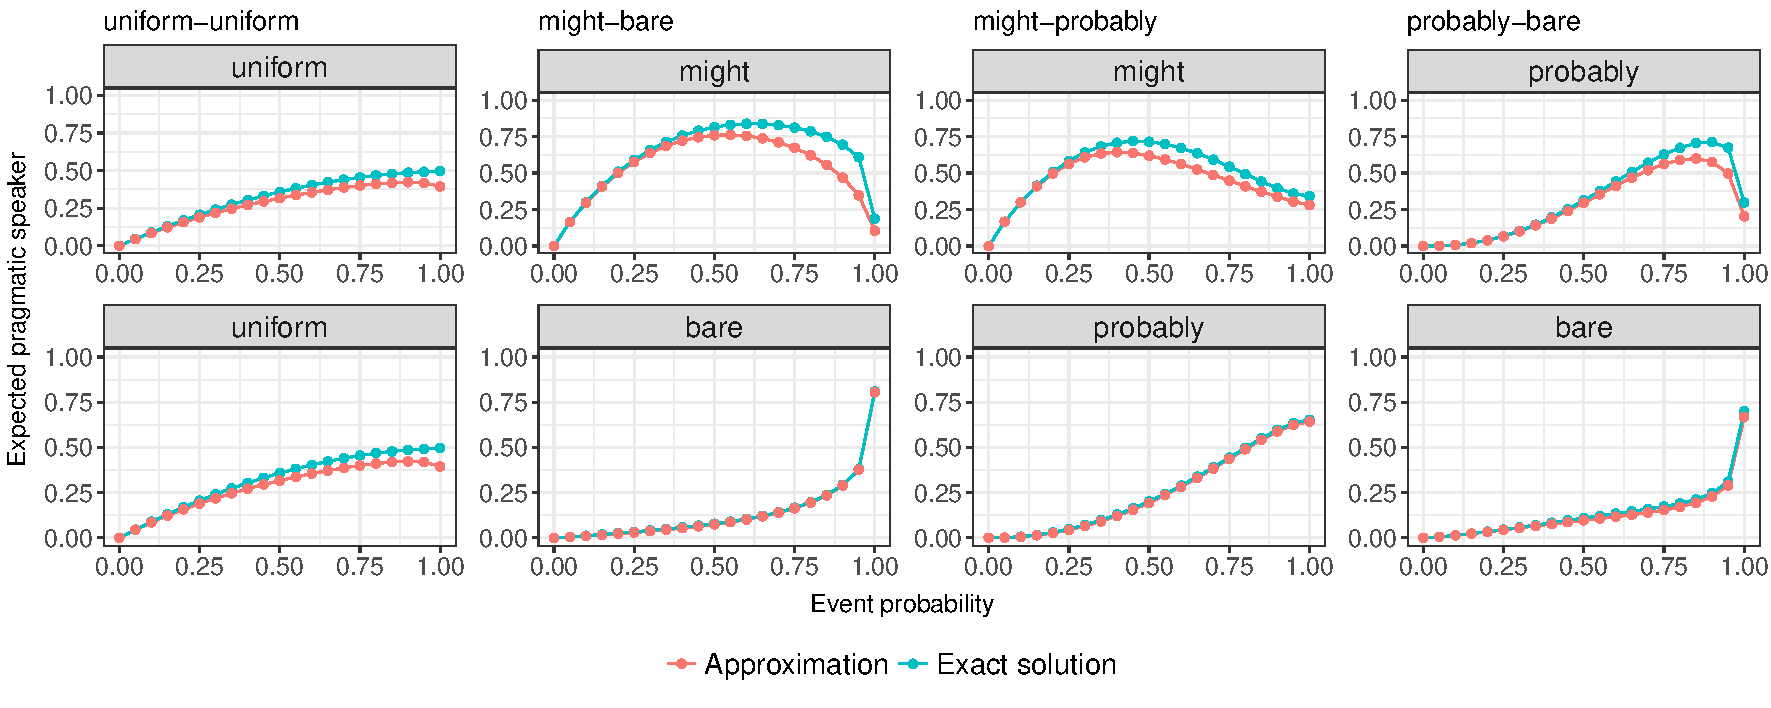
\includegraphics[width=\textwidth]{plots/fig-C1-approx-simulations.pdf}
\caption{Predictions of exact and approximate expected pragmatic speaker model for different combinations of thresholds. The leftmost panels (uniform) shows predictions of both models if both utterances have uniform threshold distributions, i.e., threshold distributions with very high variance. The other panels show model predictions under the assumption that the utterances have the threshold distributions that we inferred in Section~3. \label{fig:approx-simulations}}
\end{figure}

This approximation leads to identical results as $ES_1$ if each threshold distributions assigns all probability mass to one value, 
i.e., if we have point estimates for thresholds. To assess how much $ES_1$ and its approximation, $\widetilde{ES_1}$ deviate when 
the threshold distributions have non-zero variance, we performed several simulations, with different threshold distributions. For these
simulations, we assume that there are only two possible utterances, which makes the computation of $ES_1$ tractable.

Figure~\ref{fig:approx-simulations} shows the results of these simulations. As these plots show, the approximate model $\widetilde{ES_1}$ is a very close approximation of the expected
pragmatic speaker model $ES_1$, which suggests that this approximation should only minimally affect our modeling results. 

The model is implemented in Python using the scikit-learn \parencite{Scikit2011} and numpy \parencite{vanderWalt2011} libraries.

\chapter{Additional model predictions}


Figures~\ref{fig:norming-results-model-1} and \ref{fig:norming-results-model-2} show the model predictions and the results from all conditions in Experiment~1. 

\begin{figure}[h!]
\includegraphics[width=0.95\textwidth]{plots/fig-D1-pre\string_test\string_model\string_s1.pdf}
\caption{Model predictions and results of Experiment~1 -- Part 1. Error bars correspond to 95\% high density intervals (model predictions) and bootstrapped 95\%-confidence intervals (observed results). \label{fig:norming-results-model-1}}

\end{figure}

\begin{figure}[h!]
\includegraphics[width=0.95\textwidth]{plots/fig-D2-pre\string_test\string_model\string_s2.pdf}
\caption{Model predictions and results of Experiment~1  -- Part 2. Error bars correspond to 95\% high density intervals (model predictions) and bootstrapped 95\%-confidence intervals (observed results). \label{fig:norming-results-model-2}}

\end{figure}



\chapter[Original adaptation experiment]{Original production expectation adaptation experiment}


We originally ran a different version of the production expectation experiment which included a potential confound because the number of utterances
with each uncertainty expression was not matched across conditions. Qualitatively, this lead to the same results as Experiment~2 in the main text 
but from this experiment, it remained unclear whether the different post-exposure ratings were a result of the different number of exposure trials
across conditions or a result of listeners updating the mapping between uncertainty expressions and event likelihoods.  

For transparency, we report the procedure and the results of the original experiment here. The procedure, materials and analyses were pre-registered at \url{https://osf.io/w926x/}.

\section{Method}
\subsection{Participants}
We recruited a total of 80 participants (40 per condition) on Amazon Mechanical Turk. 
We required participants to have a US-based IP address and a minimal approval rating 
of 95\%. Participants were paid \$2 which amounted to an hourly wage of approximately 
\$12--\$15. None of the participants had previously participated in Experiment~1.

\subsection{Materials and procedure}

Materials and procedure were identical to Experiment~2. The only difference between Experiment~2 and this experiment were the number of filler trials with the other uncertainty expression, as shown in Table~\ref{tbl:materials-comparison}.

\begin{table}
\centering
\begin{tabular}{l c c c c c c | c c c c c c}
\toprule
& \multicolumn{6}{c | }{Original experiment} & \multicolumn{6}{c}{Experiment 2} \\
\midrule
& \multicolumn{2}{c}{\sc might} & \multicolumn{2}{c}{\sc probably} & \multicolumn{2}{c |}{\sc bare} & \multicolumn{2}{c}{\sc might} & \multicolumn{2}{c}{\sc probably} & \multicolumn{2}{c}{\sc bare} \\
& $n$ & $\phi$ & $n$ & $\phi$ & $n$ & $\phi$ & $n$ & $\phi$ & $n$ & $\phi$ & $n$ & $\phi$\\
\midrule
\emph{cautious} & {\bf 10} & {\bf 60\%} & 5 & 90\% & 5 & 100\% & {\bf 10} & {\bf 60\%} & 10 & 90\% & 5 & 100\% \\
\emph{confident} & 5 & 25\% & {\bf 10}  & {\bf 60\%} & 5  & 100\% & 10 & 25\% & {\bf 10}  & {\bf 60\%} & 5  & 100\% \\  
\bottomrule
\end{tabular}

\caption{Number of exposure trials ($n$) per utterance ({\sc might}, {\sc probably}, {\sc bare}) 
and associated proportion of target color gumballs ($\phi$) in the \emph{cautious} vs.~\emph{confident} 
speaker conditions in this original experiment and  Experiments~2. Critical trials bolded. \label{tbl:materials-comparison}}

\end{table}

\subsection{Exclusions} We excluded participants who provided incorrect responses to more than 3 of the attention checks. Based on this criterion, we excluded 11 participants in the \textit{confident speaker} condition and 8 participants in the \textit{cautious speaker} condition. None of the results reported below depend on these exclusions.


\section{Analysis and predictions}  

As in Experiment~2, we tested whether listeners updated their expectations after exposure by computing the difference between the AUC of the spline for 
{\sc might} and of the spline for {\sc probably} for each participant. We predicted that the mean AUC difference would be larger in the 
\emph{cautious speaker} condition than in the \emph{confident speaker} condition.

\section{Results and discussion}

\begin{figure}
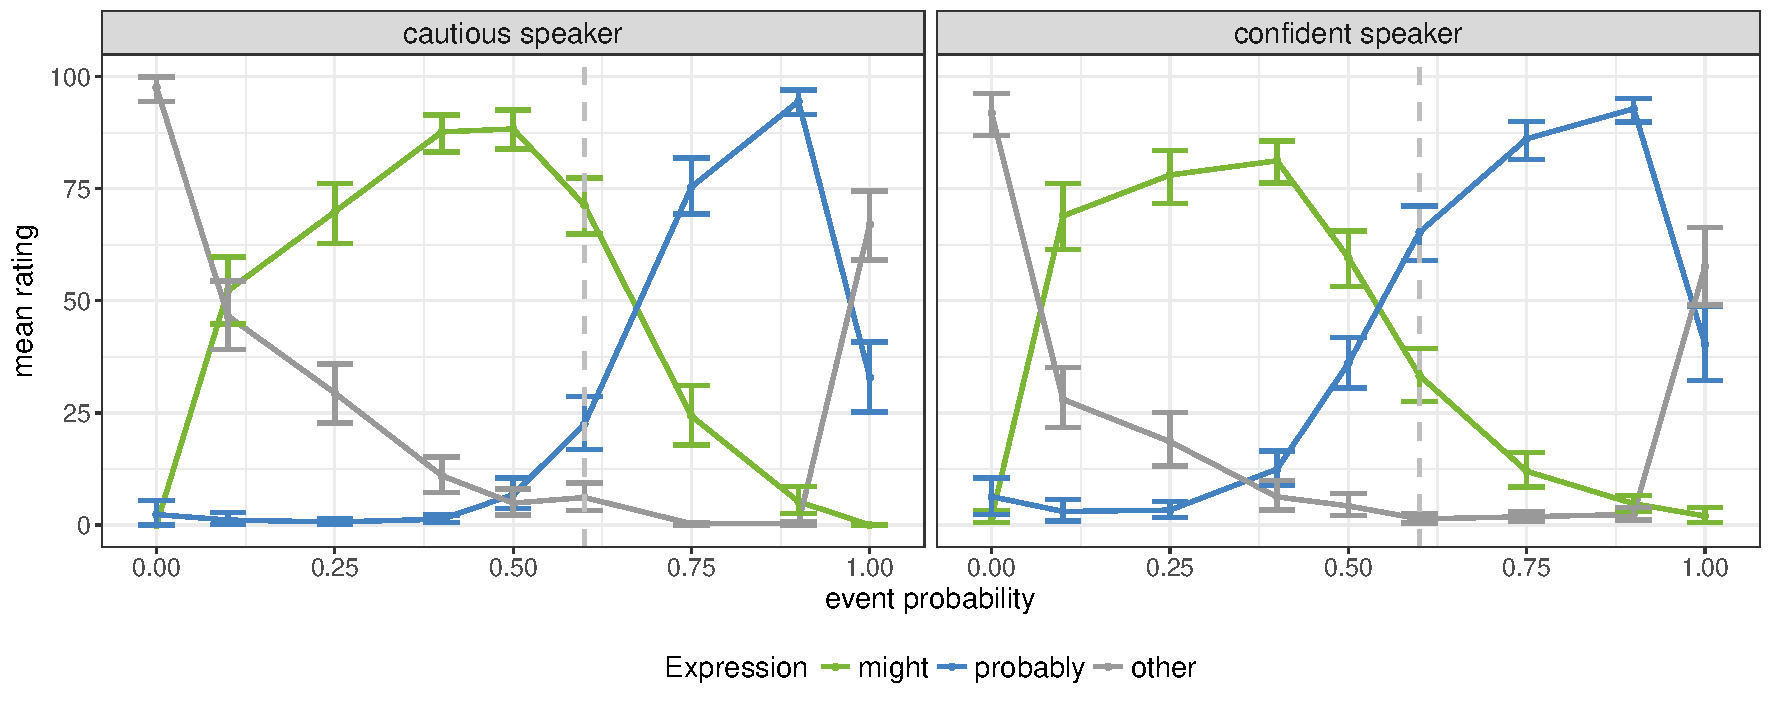
\includegraphics[width=\textwidth]{plots/fig-E1-exp-1-ratings.pdf}
\caption{Mean post-exposure ratings from original production expectation experiment. Error bars correspond to bootstrapped 95\%-confidence intervals.  The grey dotted line highlights the ratings for the 60\% event probability ratings.  \label{fig:adaptation-results-prod-orig}}
\end{figure}

\begin{figure}
\center
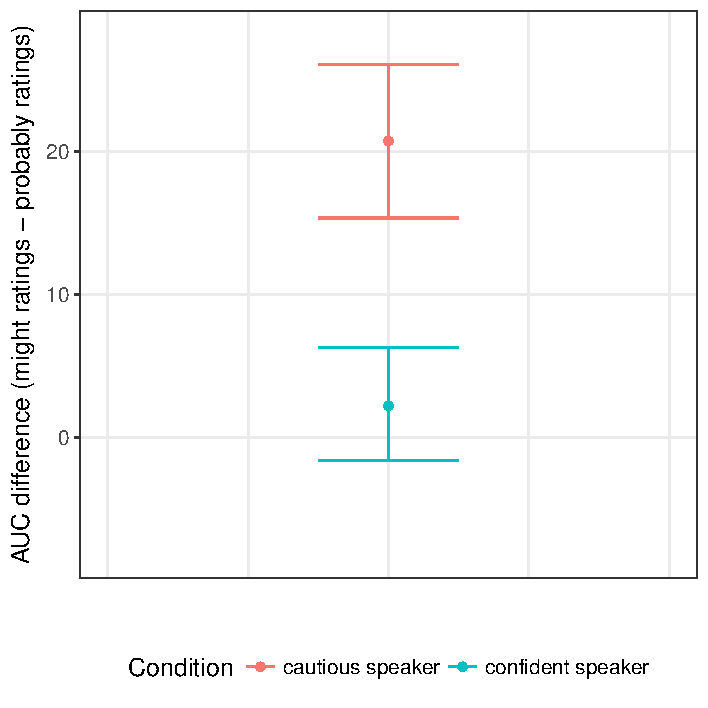
\includegraphics[width=.4\textwidth]{plots/fig-E2-exp-1-auc-orig.pdf}
\caption{Area under the curve (AUC) differences from original production expectation experiment. Error bars correspond to bootstrapped 95\%-confidence intervals.  \label{fig:adaptation-auc-prod-orig}}
\end{figure}

This experiment yielded the same results as Experiment~2. As the panels in Figure~\ref{fig:adaptation-results-prod-orig} show, participants updated their expectations about the speaker's language use and therefore made different predictions about how the speaker would use uncertainty expressions. In the \emph{cautious speaker} condition, participants gave high ratings for {\sc might} for a larger range of event probabilities than in the \emph{confident speaker} condition. On the other hand, participants gave high ratings for {\sc probably} for a larger range of gumball proportions in the \emph{confident speaker} condition than in the \emph{cautious speaker} condition. These differences result in a significantly larger AUC difference in the \emph{cautious speaker} condition than in the \emph{confident speaker} condition ($t(59) = 4.98$, $p < 0.001$, see also left panel of Figure~\ref{fig:adaptation-auc-prod-orig}).

However, from these results it remains unclear whether listeners update their expectations about the mapping between uncertainty expressions and event likelihoods. In this experiment, the number of utterances with \textit{might} and \textit{probably} differed across conditions. It is therefore possible that participants only learned that the {\it cautious speaker} overall prefers to use {\it might} and the {\it confident speaker} prefers {\it probably}. To address this confound, we conducted Experiment~2 which is reported in the main text.

\chapter[Original adaptation experiment simulations]{Model simulations for original production expectation experiment}


\begin{table}
\center
\begin{tabular}{r | c | c }
Model &   odds  &  $R^2$ \\ \midrule
fixed & $10^{-1137}$ &  0.746       \\
cost & $10^{-386}$ & 0.766     \\
threshold distributions & $10^{-207}$ &  0.856 \\
cost \& threshold distributions & 1 &  0.809 \\
\end{tabular}
\caption{Model evaluation results on data from original production expectation experiment.   \textit{odds} are the posterior likelihood odds of the models compared to the \textit{cost and threshold distributions} model.  $R$\textsuperscript{$2$} are computed between  the mean post-exposure ratings and the mean model predictions. \label{tbl:model-comparison-orig}}
\end{table}


Table~\ref{tbl:model-comparison-orig} shows the results of the model comparison  for the original production expectation experiment and  Figures~\ref{fig:post-exposure-model-original}, \ref{fig:post-exposure-thresholds-original}, and \ref{fig:post-exposure-costs-original} show the posterior predictions
of the model simulations, the post-adaptation threshold distributions, and the post-adaptation costs, respectively. For these simulations, we took the MAP variance parameters that we estimated for the data from Experiment~2, so we did not fit any parameters to the data from the original production expectation experiment. In each condition, the model was exposed to the 20 utterances that participants were exposed to in the experiment (see left part of Table~\ref{tbl:materials-comparison}).

These modeling results further demonstrate the stability of the results reported in the main text. We again find that the \textit{cost \& threshold distributions} model predicts the post-exposure data best according to the posterior odds metric, and the inferred post-exposure threshold distributions and cost values exhibit the same patterns as we found in the simulations for Experiment~2. Not surprisingly, the inferred cost differences between \textit{might} and \textit{probably} are bigger in the present simulations for the original experiment reflecting that the exposure across conditions was not balanced. 

However, as shown in Table~\ref{tbl:model-comparison-orig}, we also find that according to the $R^2$ metric, the model according to which listeners only update their beliefs about threshold distributions predicts the post-exposure
behavior better than the  \textit{cost \& threshold distributions} model. While we generally expect the ranking of models to be the same according to both metrics, we explained in the main text that in our setup, multiple assumptions
of the $R^2$ metric are violated and therefore, we do not consider the ranking of models according to the $R^2$ metric as evidence that listeners only update beliefs about threshold distributions -- especially given that in all other simulations, both metrics suggested that listeners update both types of representations.





\begin{figure}[h!]
  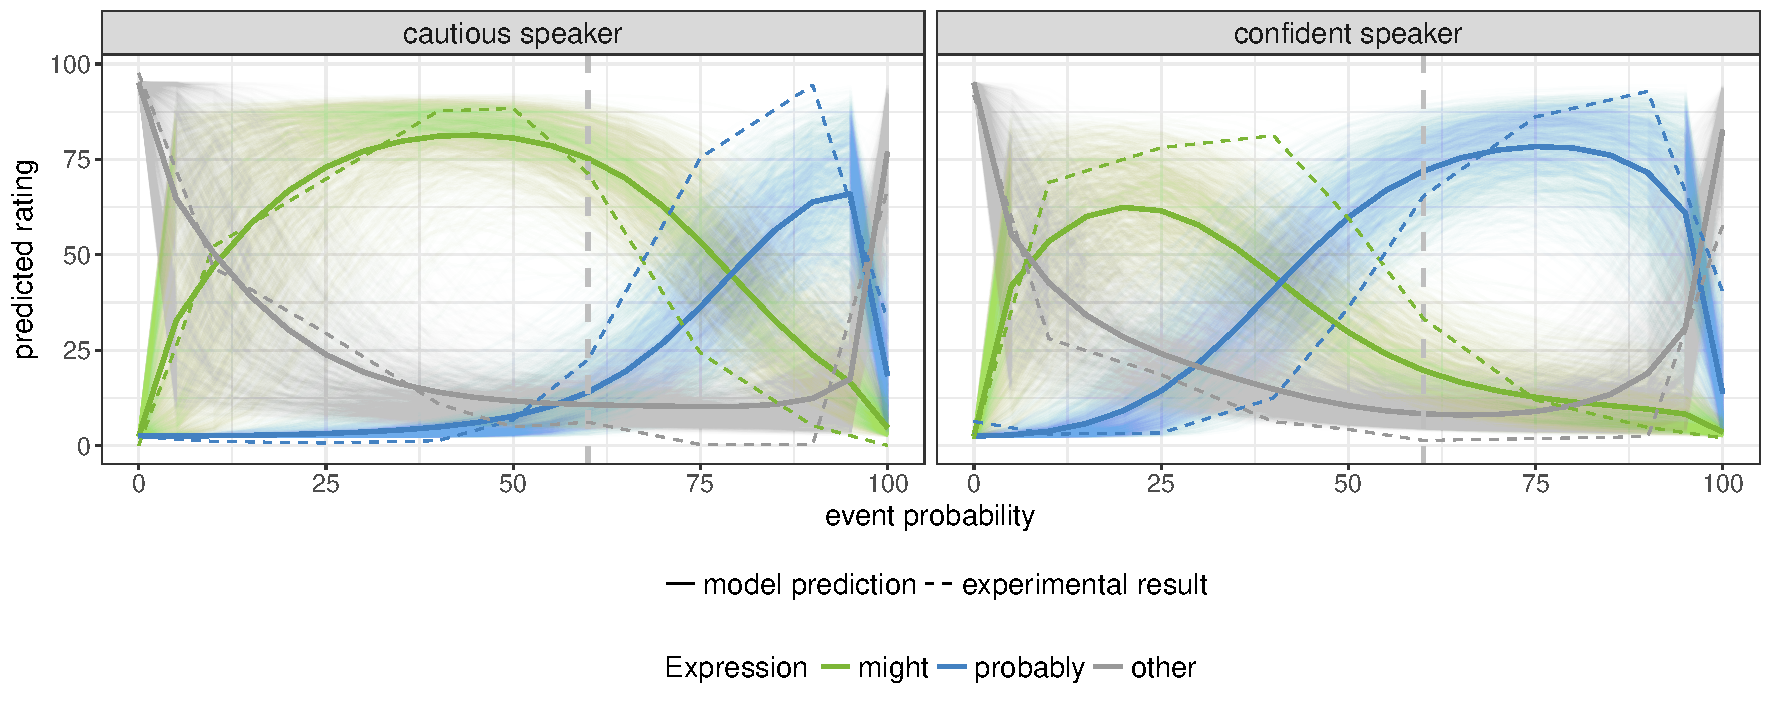
\includegraphics[width=\textwidth]{plots/fig-F1-adaptation-posterior-predictions.pdf}
  \caption{Post-adaptation model predictions from simulations for original production expectation experiment and experimental results. 
  The solid lines shows the mean model predictions and the thin lines around the mean show the distribution of model predictions. \label{fig:post-exposure-model-original}}
\end{figure}

\begin{figure}[h!]
  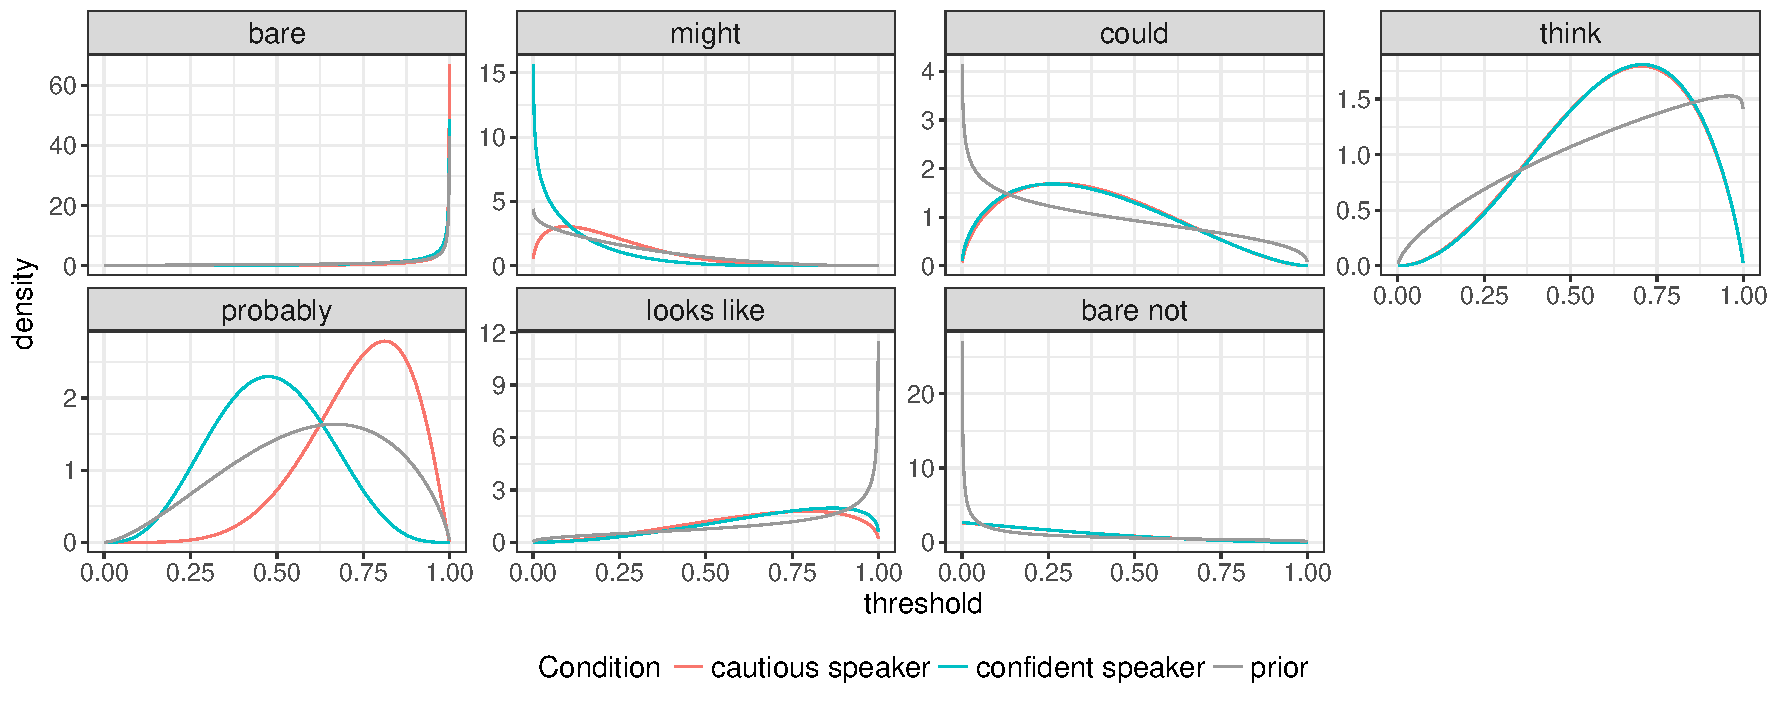
\includegraphics[width=\textwidth]{plots/fig-F2-adaptation-posterior-thresholds.pdf}
  \caption{Post-adaptation threshold distributions from the simulations for original production expectation experiment. \label{fig:post-exposure-thresholds-original}}
\end{figure}

\begin{figure}[h!]
\center
  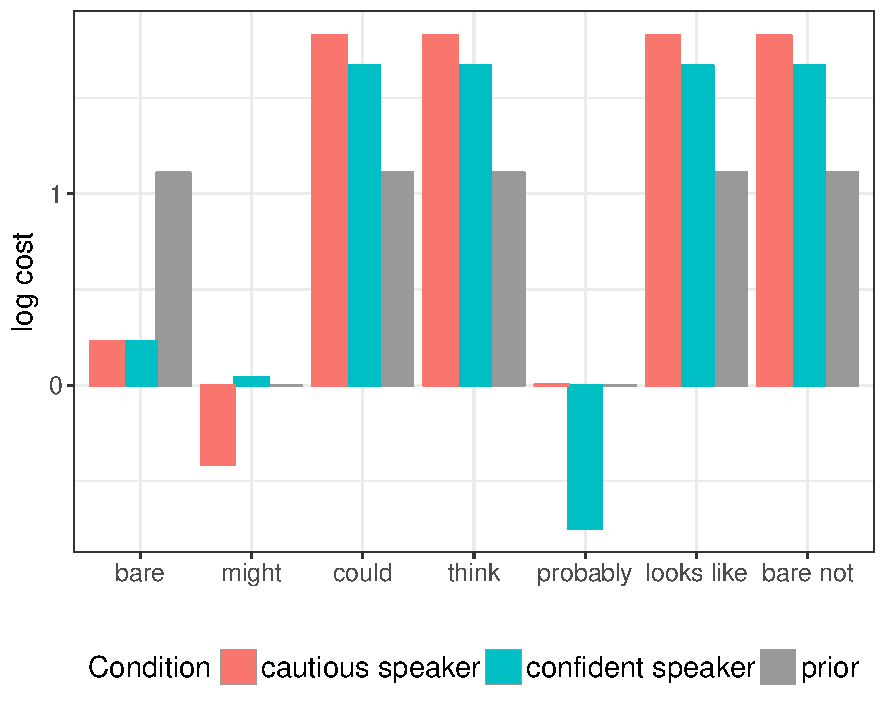
\includegraphics[width=0.5\textwidth]{plots/fig-F3-adaptation-posterior-costs.pdf}
  \caption{Post-adaptation $log$ cost values from simulations for for original production expectation experiment. Note that the cost of \textsc{might} and \textsc{probably} 
  in the norming data model was 1 and therefore the $log$ cost for these utterances is 0.  \label{fig:post-exposure-costs-original}}
\end{figure}




\chapter{Original interpretation experiment}

As we mentioned in the main text, we originally ran a slightly different version of the comprehension experiment in which participants used sliders to rate which gumball machine they thought the speaker was describing. While the results were qualitatively the same as in the experiment reported in the main body of the paper, the use of sliders seemed to confuse some participants (see details below) and therefore we changed the procedure such that participants provided ratings by distributing coins. For transparency, we report the 
procedure and the results of the original experiment here.

\subsection{Method}
\subsubsection{Participants}

We recruited a total of 80 participants (40 per condition) on Amazon Mechanical Turk. We required participants to have a US-based IP address and a minimal approval rating of 95\%. Participants were paid \$2 which amounted to an hourly wage of approximately \$10--\$12. None of the participants had participated in any of the previous experiments. 

\subsubsection{Materials and Procedure}

The exposure phase was identical as in the other adaptation experiments: participants were either exposed to a 
\textit{cautious} speaker or a \textit{confident} speaker. Six of the exposure trials included attention checks in which
participants had to indicate whether they saw a grey X on the previous trial or not.

Similar to Experiment~3, the test trials probed participants'
interpretations of the utterances {\sc might}, {\sc probably}, and {\sc bare}. On test trials, participants listened
to a recording of the speaker they encountered during the exposure phase and then rated how likely they
thought it was that the speaker saw different gumball machines. On each trial, like in Experiment~3, participants
provided ratings for 9 gumball machines. However, unlike in Experiment~3, participants indicated their ratings
by adjusting 9 sliders. Participants completed 6 test trials in total -- one for each expression-color pair.

\subsubsection{Exclusions}

We excluded participants who failed more than 2 out of 6 attention checks, which led to 2 exclusions in the \emph{cautious speaker} condition and 1 exclusion in the \emph{confident speaker} condition.


\subsection{Analysis and Predictions}

As for Experiment~3, we expected that listeners interpret a more confident speaker's utterance 
to communicate a lower event probability than a more cautious speaker's utterance. We measured
the interpretation of utterances by normalizing the ratings across the 9 gumball machines so that they sum to
1 and then computing the expected value for the proportion of blue and orange gumballs. 
We predicted that the expected values of target color gumball proportions after hearing {\sc might} and {\sc probably} 
were going to be larger in the \emph{cautious speaker} condition than in the \emph{confident speaker} condition.

\subsection{Results and Discussion}

\begin{figure}[h!]
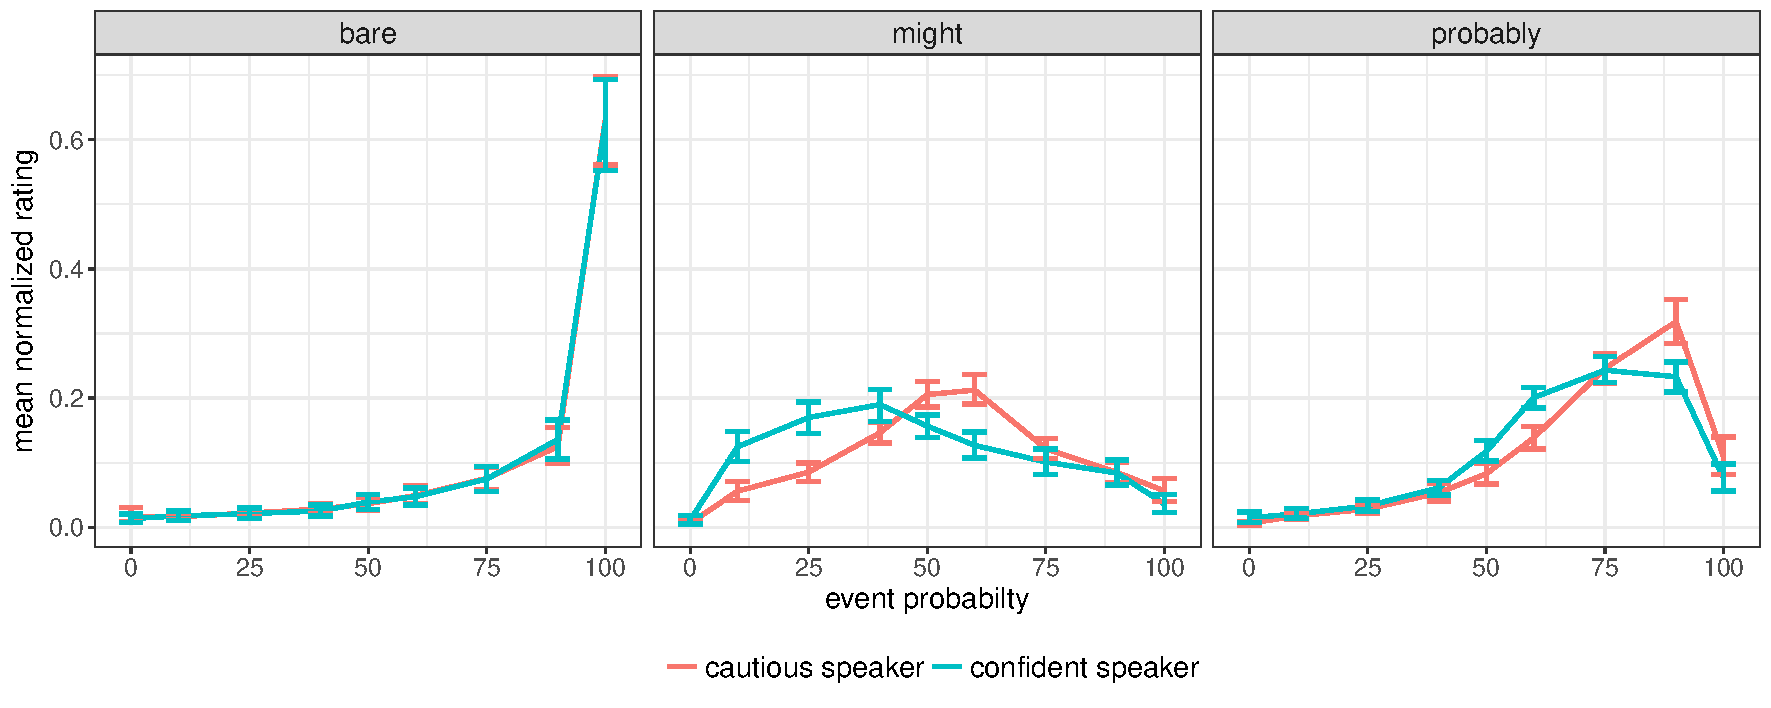
\includegraphics[width=\textwidth]{plots/fig-G1-exp-2-ratings-orig.pdf}
\caption{Aggregated post-exposure ratings from the original interpretation experiment.  \label{fig:adaptation-results-comp-orig}}
\end{figure}

Figure~\ref{fig:adaptation-results-comp-orig} shows the aggregated and normalized ratings for the two conditions.  As predicted, participants provided higher ratings for gumball machines with higher target color percentages after hearing {\sc might} and {\sc probably} in the \emph{cautious speaker} condition than in the \emph{cautious speaker} condition. This also led to a significantly higher expected value for {\sc might} ($t(75)=3.05$, $p<0.01$) and {\sc probably} ($t(75)=3.08$, $p<0.01$) in the \emph{cautious speaker} condition as compared to the \emph{confident speaker} condition.

This means that qualitatively, the results are the same as in Experiment~3. However, since participants had the option to assign high 
ratings to 
all gumball machines (they could assign a maximum rating to each gumball machine if they wanted to), we noticed that many participants assigned very high ratings to most gumball 
machines and therefore did not indicate their interpretation of the utterance. Further, it seemed that some participants
understood the instructions as rating the likelihood of getting a target color gumball and provided ratings proportional to the 
target color gumball proportion independent of the utterance. For these reasons, we revised the original paradigm as described
in the main text and asked participants to indicate their interpretation using a limited set of coins, which appeared to be less
confusing for participants. 
